\appendixsection{Граф состояний интеллектуального агента}

Граф состояний интеллектуального агента, реализованный в модуле \texttt{graph.py}, содержит двадцать один узел, объединённый в семь функциональных фаз, и все условные переходы между ними. Полная схема графа приведена на рисунке~\ref{fig:state-graph}.

Условные обозначения. Узлы графа изображены прямоугольниками со скруглёнными углами и подписаны идентификатором в исходном коде и кратким русским описанием выполняемой операции. Терминальные состояния обозначены кругами: заполненный чёрный круг~--- начальное состояние (входящее сообщение пользователя), круг с точкой внутри~--- допустимое конечное состояние (любой из возможных ответов пользователю). Узел \texttt{ask\_clarification} выделен формой <<заметка>>: он приостанавливает обработку и удерживает поток в ожидании ответа пользователя. Узлы сгруппированы в семь окрашенных подграфов по функциональным фазам: жёлтый~--- маршрутизация и контроль тарифа; оранжевый~--- обработка дополнительных вопросов; фиолетовый~--- точечная правка готового договора; зелёный~--- классификация сделки; синий~--- проверка общих норм и поиск специальных; светло-жёлтый~--- проверки формы и достаточности данных; розовый~--- генерация и итеративная валидация; бирюзовый~--- формирование рекомендаций и сохранение результата. Сплошные стрелки изображают безусловные и условные переходы между узлами, подписи на стрелках раскрывают предикат соответствующего перехода. Пунктирные стрелки оранжево-красного цвета выделены отдельно и обозначают переходы, прерывающие обработку графа для диалогового уточнения у пользователя~--- ответ пользователя возобновляет обработку в соответствующем узле проверки. Пунктирная циклическая стрелка из узла \texttt{followup\_subagent\_search} в самого себя обозначает итеративный цикл изолированного поиска по корпусу до достижения целевого ответа или исчерпания лимита попыток.

\landscapestart

\begin{figure}[H]
\centering
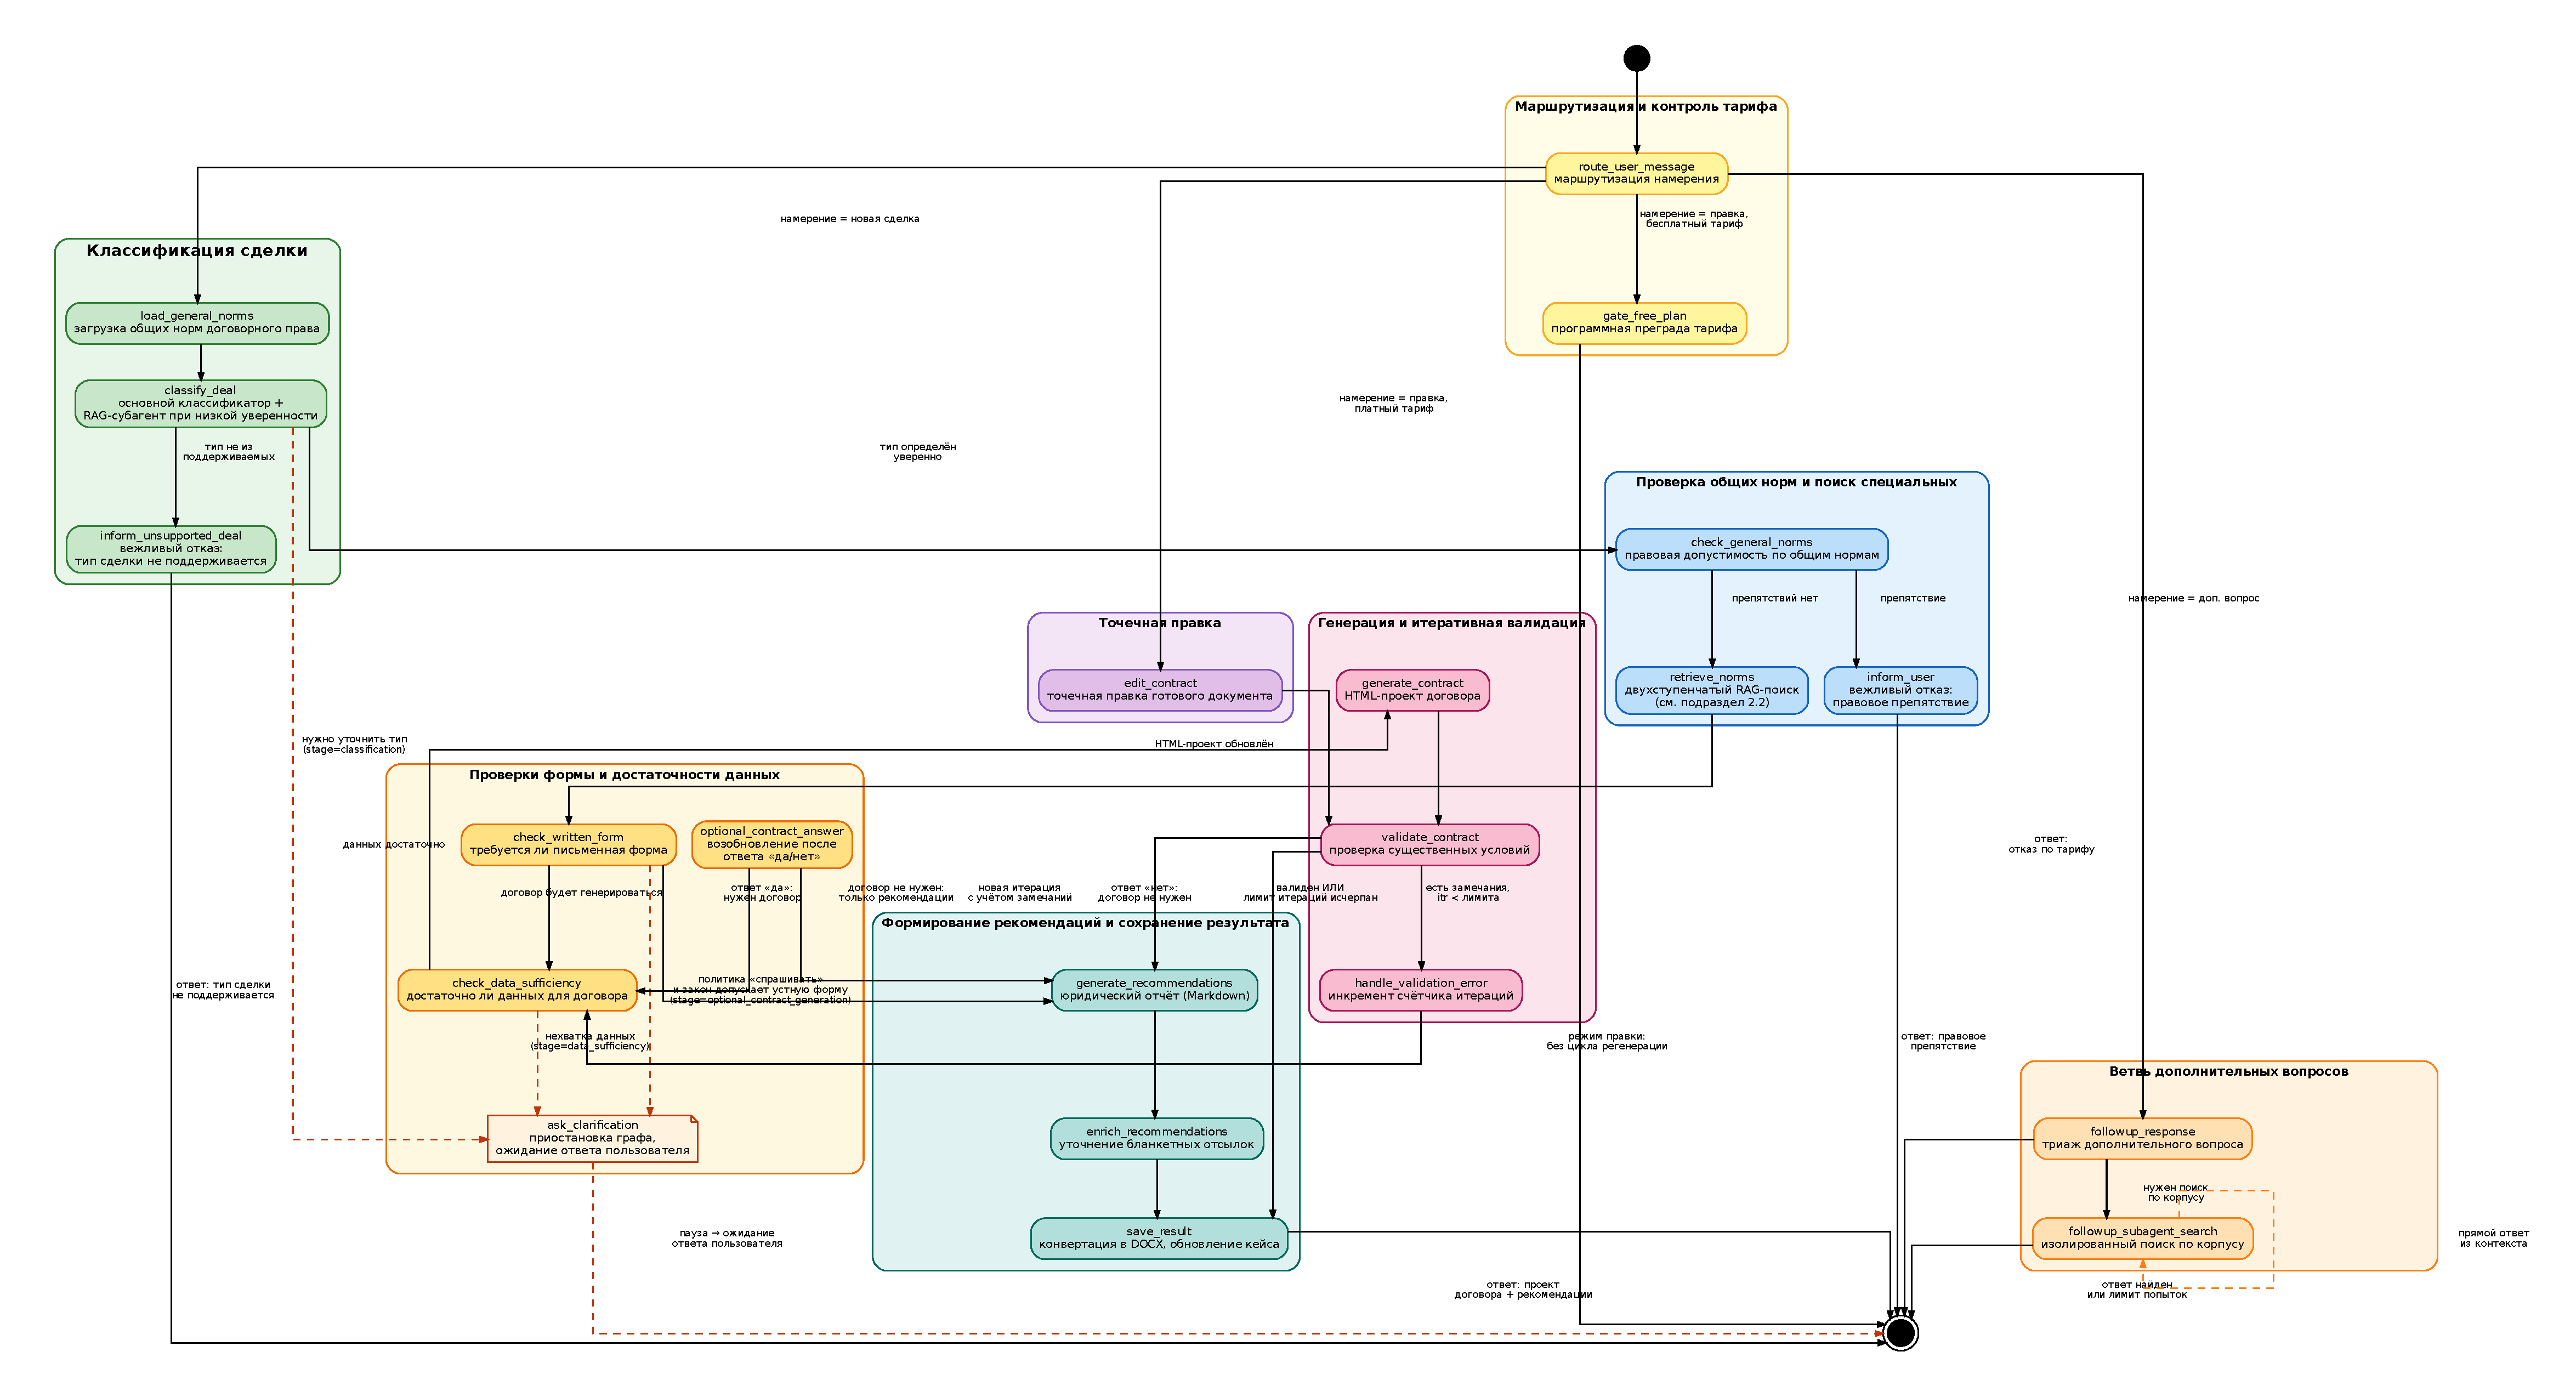
\includegraphics[width=\linewidth,height=0.92\textheight,keepaspectratio]{inc/state_graph}
\caption{Граф состояний интеллектуального агента: основной путь подготовки документа, вспомогательные ветви (программная преграда тарифа, точечная правка договора, обработка дополнительных вопросов) и точки диалогового уточнения у пользователя}
\label{fig:state-graph}
\end{figure}

\landscapestop
